\subsection{Anforderungen und Rahmenbedingungen}

Dieser Abschnitt beschreibt die Anforderungen an das Softwaresystem mittels Anwendungsfällen und 
beschreibt die technischen Rahmenbedingungen, in dem das Softwaresystem eingebettet ist.

Die Anwendungsfälle beschreiben die Arbeit mit dem \textit{One-Million-Song}-Datensatz. Dieser Datensatz
enthält im original in etwa $300$ Gigabyte an Daten von Musikstücken, bei dem pro Musikstück über $100$ Attribute pro Song
angegeben sind. Aufgrund seiner Größe eignet sich dieser Datensatz für die Untersuchung von
Big-Data-Anwendungen.

Das Anwendungsfalldiagramm \ref{anforderungen:usecasediagramm} zeigt in  der Übersicht aller Anwendungsfälle für
den Arbeit mit dem Million-Song-Datensatz auf dem Cluster.

\begin{figure}
	\centering
	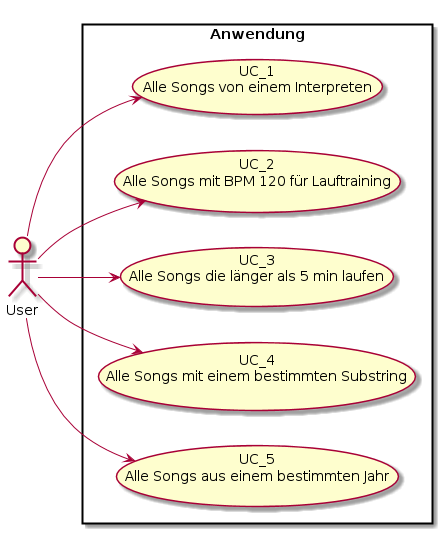
\includegraphics[width=0.5\textwidth]{images/useCaseDiagramm.png}
	\caption{Anwendungsfall-Diagramm, UML 2.0. Alle Anwendungsfälle für das Million-Song-Projekt}
	\label{anforderungen:usecasediagramm}
\end{figure}

Es folgt eine kurze Beschreibung der einzelnen Anwendungsfälle. Auf eine detaillierte Ausarbeitung im Rahmen einer 
ausführlichen Anforderungsanalyse soll in diesem Falle verzichtet werden, weil ein konkretes Anwendungsszenario fehlt und
die Anwendungsfälle künstlicher Natur sind, um den Einsatz von Hadoop, MapReduce und Hbase im Bereich der
Big-Data-Anwendungen zu evaluieren.

\begin{description}
	\item[UC 1] Der Nutzer möchte den Namen aller Musikstücke, die ein bestimmter Interpret geschrieben hat.
	\item[UC 2] Der Nutzer möchte für sein Lauftraining nur den Namen jener Musikstücke haben, die eine Beats-Per-Minute-Rate
		von 120 haben.
	\item[UC 3] Der Nutzer möchte den Namen aller Musikstücke, die länger als 5 Minuten am Stück laufen.
	\item[UC 4] Der Nutzer möchte ein oder mehrere Musikstücke eines bestimmten Namens. Dabei muss der Name nicht dem 
		kompletten Musiktitel beschreiben.
	\item[UC 4] Der Nutzer möchte die Namen aller Musikstücke erhalten, die in einem bestimmten Jahr zum ersten Mal erschienen sind.
\end{description}

Die Rahmenbedingungen teilen sich in die Hardware-Rahmenbedingungen und in die Software-Rahmenbedingungen auf.
Die Hardware, die uns zur Verfügung gestellt wurde besteht aus einem Verbund von 5 homogenen Server-Rechnern, 
die über ein Ethernet-Netzwerk gleichwertig miteinander verknüpft sind. Physikalisch sind alle Knoten an einem gemeinsamen
Switch angeschlossen als physikalische Stern-Topologie. Dies hat aus logischer Sicht zur Folge, dass eine direkte Kommunikation
zwischen den Knoten möglich ist. Die Bandbreite des gesamten Netzwerkes ist mit 20Mbit/s angegeben, was durch die Topologie
auch zwischen den einzelnen Knoten möglich wäre.

Die Server-Knoten sind alle mit folgender Hardware ausgestattet:
\begin{itemize}
	\item Intel i7-4790K CPU
	\item 32 GB RAM
	\item 256 GB SSD
	\item 2 TB HDD
\end{itemize}

Auf der Seite der Software ist auf allen Knoten mit \textit{Ubuntu} eine Linux-Distribution in der Version 
\textit{16.04.1 LTS Server 64-Bit} installiert. Root-Rechte sind gewährt.
Anzumerken ist, dass alle Ressourcen mit 9 anderen Teams geteilt werden und alle Teams auf der selben 
Instanz des Betriebssystems arbeiten und nur durch unterschiedliche Nutzer getrennt sind. 
Diese Rahmenbedingung ist insbesondere bei der Konfiguration der Netzwerk-Ports bei verteilten Anwendungen 
zu beachten, da verschiedene Anwendungen eventuell auf dem gleichen Port lauschen und somit 
Konfikte entstehen können.